\documentclass[10pt]{article}

\usepackage[margin=1.2in]{geometry} % set margin size
\usepackage{fancyhdr}               % for headers/page numbers
\usepackage{booktabs}               % tabular settings
\usepackage{tabularx}               % better tables
\usepackage[bookmarks]{hyperref}    % additional PDF settings
\usepackage[parfill]{parskip}       % adjusting paragraph settings

\usepackage{fontspec}               % for changing the font

% change the style for the header
\pagestyle{fancyplain}
\date{}
\setlength{\headheight}{18pt}

% use system font
\setmainfont{Droid Serif}

\def\doctitle{EE 119c Project Proposal}
\hypersetup{pdftitle={\doctitle}}

\title{Real-time Hand Tracking with Neural Nets on an FPGA}
\author{%
    \begin{tabular}{cc}
        Brian Kubisiak  & <bkubisia@caltech.edu> \\
        Quinn Osha      & <qosha@caltech.edu>
    \end{tabular}
}

\begin{document}

\lhead{\large{Brian Kubisiak, Quinn Osha}}
\chead{}
\rhead{\large{\today}}

\maketitle

\thispagestyle{empty}

\section{Functional Specification}
\label{sec:functional_specification}

For our project, we will be designing and implementing a system for tracking
a hand in real time from a camera input. The system will be implemented using a
Digilent Nexys 4 FPGA development board. It will take an input from a camera
connected to the USB port, analyze the data on the Artix 7 FPGA, and output each
from over the VGA port with a cursor overlay. The cursor overlay will indicate
where in the frame the hand is located. While the neural net is computing the
hand position, the frame will temporarily be stored in the board's memory---the
FPGA is too small to process an entire frame at once.

\subsection{Operation}
\label{sub:operation}

The FPGA design will consist of three distinct layers:
\begin{description}
    \item[Input Layer] For communicating with the USB camera, writing the frame
        to memory, and converting the frame into a format that the neural net
        can use.
    \item[Neural Network] For analyzing the camera data to determine where the
        hand is in the frame.
    \item[Output Layer] For reading the frame back from memory, overlaying a
        cursor on the hand position, and generating control signals to output
        the frame through a VGA port.
\end{description}

A top-level block diagram showing the layers and their connections is shown in
figure~(\ref{fig:top-level}). The Rx and Tx inputs come from the USB-UART
bridge. The Data, Address, Wr, and Rd signals go to the memory on the Digilent
board. Note that the Data and Address buses must be muxed before connecting to
the pins. The HSYNC, VSYNC, and Data outputs will go to the VGA port on the
board.

\begin{figure}[h]
    \centering
    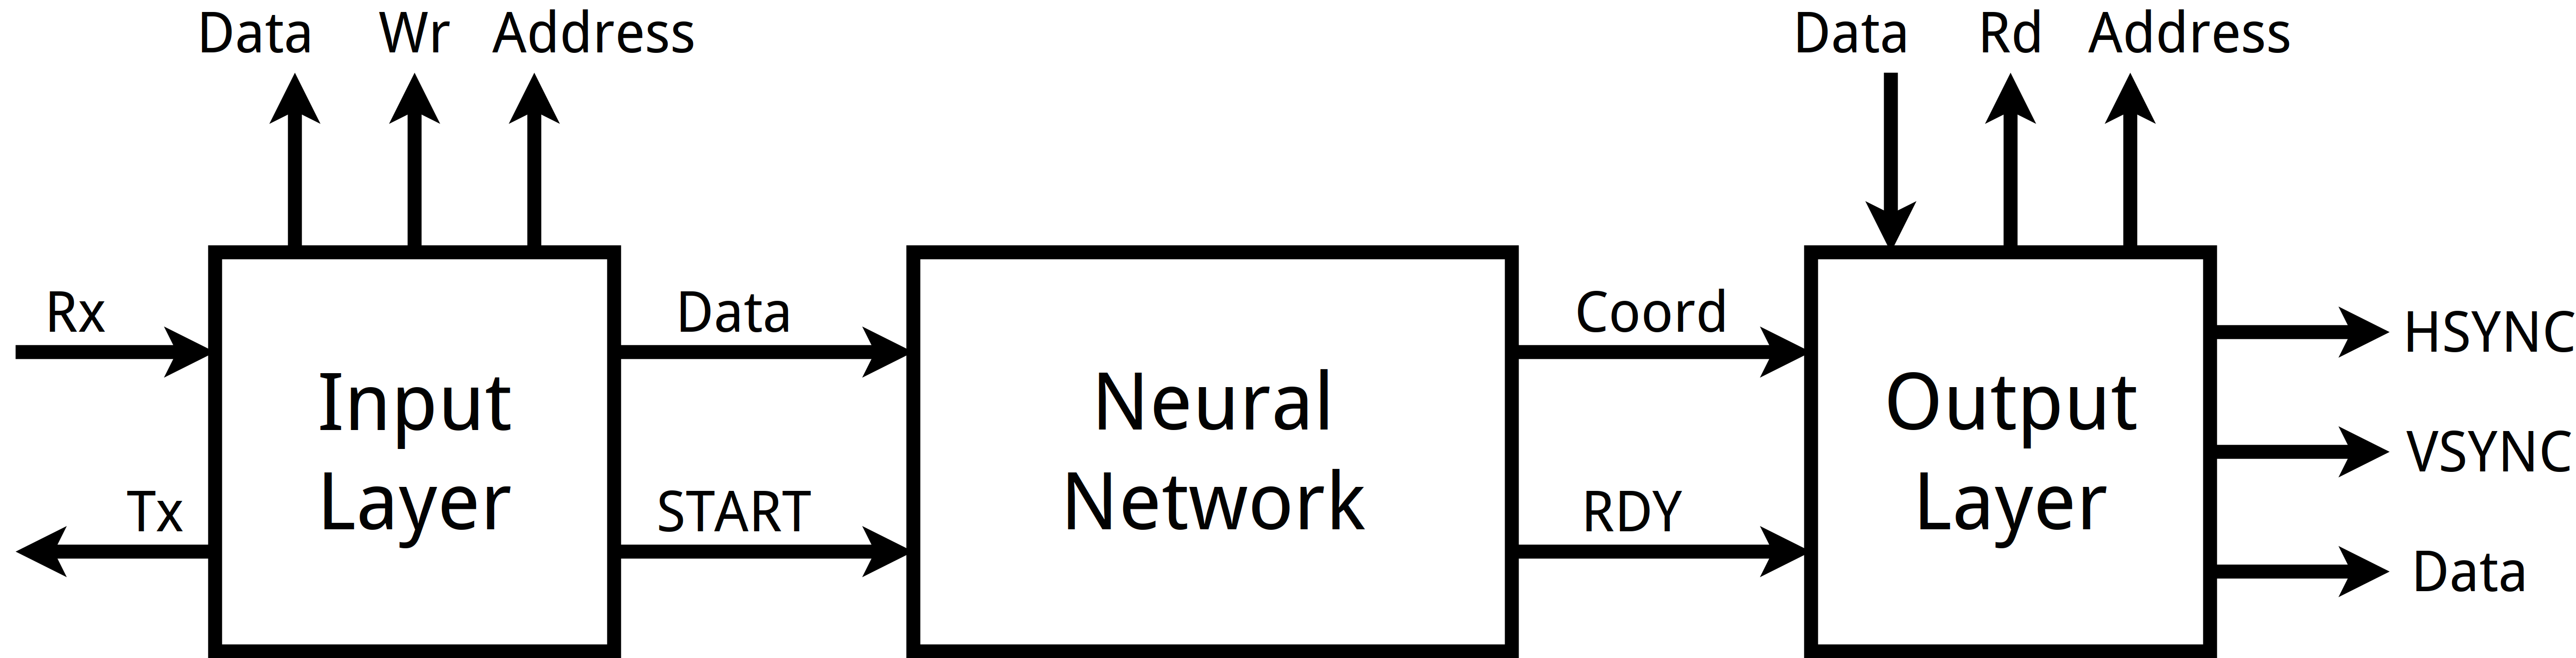
\includegraphics[width=0.8\linewidth]{diagrams/top-level.png}
    \caption{Top-level block diagram for the system.}
\label{fig:top-level}
\end{figure}

\subsubsection{Input Layer}
\label{ssub:input_layer}

\subsubsection{Neural Network}
\label{ssub:neural_network}

\subsubsection{Output Layer}
\label{ssub:output_layer}

The USB controller will load each pixel serially from the camera, storing the
pixel in a shift register. Once the pixel is completely shifted into the
controller, the controller will output the pixel (in parallel) to the input
frame buffer.

This input frame buffer will act like a FIFO for loading data from the USB
controller. Once the buffer is full, it will output the data in parallel
to both the neural net and the output buffer. Once this data is sent to the
neural net and output buffer for processing, the USB controller can begin
loading new data into the input buffer.

The output buffer will have two inputs: the first input will be a massively
parallel input for loading all the data from the input buffer. The second input
will allow individual pixels to be reset. This will be connected to the cursor
drawing logic in order to draw the cursor at the hand's location.

The neural network will load all the data in parallel from the input buffer and
operate on the data using the machine-learned parameters to find the coordinates
of the hand that is being tracked. These coordinates will then be output to the
cursor drawing logic. The cursor drawing logic will accept the coordinates
produced by the neural net and will output control signals to the output buffer
for drawing the cursor.

The output buffer---after loading the input data and having the cursor drawn to
it---will output one pixel at a time to the VGA controller. The VGA controller
will load this data into a shift register, then shift it out to the display
(along with the needed control signals). Due to the separate input and output
buffers, a frame can be input while the previous frame is being shifted out.

\subsection{Algorithms}
\label{sub:algorithms}

We will be using a convolutional neural network to identify where the hand is
located in each frame. The parameters for the neural network will be learned in
advance on the computer, then hard-coded into the FPGA neural net.
Time-permitting, we will also implement unsupervised learning on the FPGA in
order to allow the system to learn without hard-coded parameters.

\subsection{Inputs}
\label{sub:inputs}

The input to this system will be video input through a USB controller. Each
frame that is input to the USB controller will be stored in an internal frame
buffer before being processed by the neural net.

\subsection{Outputs}
\label{sub:outputs}

The output from this system will be through a VGA controller. The VGA output
will be taken from an output frame buffer. The output frame will be generated
from the input frame with a cursor overlaid on the position of the hand
(identified by the neural net).

\section{Schedule}
\label{sec:schedule}

\setlength\extrarowheight{3pt}
\begin{tabularx}{\textwidth}{c X}
    Date & Tasks \\
    \midrule
    4/7--4/13 & Research current implementations of neural nets on FPGAs. Decide
    on video input and output devices (size and pixel depth). Write code for USB
    controller. \\
    4/14--4/20 & Write code for input data buffer and input data handling.
    Design---in a high-level-language---the desired neural net. \\
    4/21--4/27 & Test and configure the neural net on the computer. Write code
    for output data buffer and handling. \\
    4/28--5/4 & Begin coding the neural net on the FPGA\@. Write code for output
    display handling using VGA\@. \\
    5/5--5/11 & Finish coding the neural net. \\
    5/12--5/18 & Write code for the cursor video output. That is, given x and y
    coordinates, print the cursor at that point. \\
    5/19--5/25 & Write the top-level entity for the system, combining all the
    blocks. Train (unsupervised) the neural net. \\
    5/26--6/1 & Finish training the neural net. Fix any other bugs/issues. \\
    6/2--6/5 & Finish documentation and final touches.
\end{tabularx}

\section{Demonstration}
\label{sec:demonstration}

This system will be demonstrated by attaching a video camera to the USB input
and a monitor to the VGA output. Then, the system should detect a hand in the
input frame and output the frame to the monitor with a cursor overlaid on the
position of the hand.

\end{document}

